%\documentclass[border=5mm,tikz]{standalone}
\usetikzlibrary{calc}
%\begin{document}
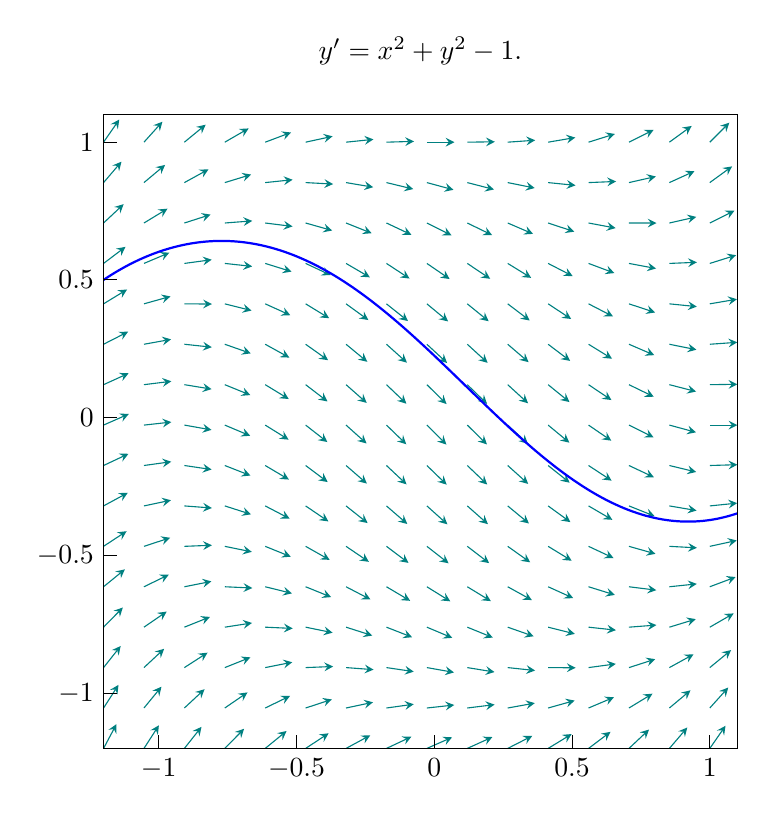
\begin{tikzpicture}[declare function={f(\x,\y)=\x*\x+\y*\y-1;},scale=3.5]
\def\xmax{1} \def\xmin{-1.2}
\def\ymax{1} \def\ymin{-1.2}
\def\nx{15}  \def\ny{15}

\pgfmathsetmacro{\hx}{(\xmax-\xmin)/\nx}
\pgfmathsetmacro{\hy}{(\ymax-\ymin)/\ny}
\foreach \i in {0,...,\nx}
\foreach \j in {0,...,\ny}{
\draw[teal,-stealth] 
({\xmin+\i*\hx},{\ymin+\j*\hy}) -- ++ ({atan2(f({\xmin+\i*\hx},{\ymin+\j*\hy}),1)}:0.1);
}
\pgfmathsetmacro{\stepx}{0.01}
\pgfmathsetmacro{\nextx}{\xmin+\stepx}
\pgfmathsetmacro{\nextnextx}{\xmin+2*\stepx}
\pgfmathsetmacro{\xfin}{\xmax+0.1}
\xdef\lstX{(\xmin,0.5)}
\pgfmathsetmacro{\myy}{0.5}
\foreach \x in {\nextx,\nextnextx,...,\xfin}
{\pgfmathsetmacro{\myy}{\myy+f(\x,\myy)*\stepx}
\xdef\myy{\myy}
\xdef\lstX{\lstX (\x,\myy)}
}
\draw[blue,thick] plot[smooth] coordinates {\lstX};
\draw (\xmin,\ymin) rectangle ($(\xmax,\ymax)+(1mm,1mm)$);
\draw (current bounding box.north) node[above=5mm]{$y'=x^2+y^2-1$.};
\foreach \i in {-1,-0.5,0,0.5,1} 
\draw (\i,\ymin) node[below]{$\i$}--++(90:.5mm) 
(\xmin,\i) node[left]{$\i$}--++(0:.5mm);
\end{tikzpicture}
%\end{document}